\documentclass[a4paper, 14pt]{extarticle}

% Поля
%--------------------------------------
\usepackage{geometry}
\geometry{a4paper,tmargin=2cm,bmargin=2cm,lmargin=3cm,rmargin=1cm}
%--------------------------------------


%Russian-specific packages
%--------------------------------------
\usepackage[T2A]{fontenc}
\usepackage[utf8]{inputenc}
\usepackage[english, main=russian]{babel}
\usepackage{cmap}
%--------------------------------------

\usepackage{textcomp}
\usepackage{amssymb}

% Красная строка
%--------------------------------------
\usepackage{indentfirst}               
%--------------------------------------             


%Graphics
%--------------------------------------
\usepackage{graphicx}
\graphicspath{ {./images/} }
\usepackage{wrapfig}
%--------------------------------------

% Полуторный интервал
%--------------------------------------
\linespread{1.3}                    
%--------------------------------------

%Выравнивание и переносы
%--------------------------------------
% Избавляемся от переполнений
\sloppy
% Запрещаем разрыв страницы после первой строки абзаца
\clubpenalty=10000
% Запрещаем разрыв страницы после последней строки абзаца
\widowpenalty=10000
%--------------------------------------

%Списки
\usepackage{enumitem}

%Подписи
\usepackage{caption} 

%Гиперссылки
\usepackage{hyperref}

\hypersetup {
	unicode=true
}

%Рисунки
%--------------------------------------
\DeclareCaptionLabelSeparator*{emdash}{~--- }
\captionsetup[figure]{labelsep=emdash,font=onehalfspacing,position=bottom}
%--------------------------------------

\usepackage{tempora}
\usepackage{amsmath}
\usepackage[dvipsnames]{xcolor}
\usepackage{listings}
\lstset{
  belowcaptionskip=1\baselineskip,
  breaklines=true,
  frame=L,
  xleftmargin=\parindent,
  language=Java,
  showstringspaces=false,
  basicstyle=\footnotesize\ttfamily,
  keywordstyle=\bfseries\color{blue},
  commentstyle=\itshape\color{purple},
  identifierstyle=\color{black},
  stringstyle=\color{red},
  numbers=left,           
  numberstyle=\tiny\color{gray}, 
  numbersep=10pt,      
  % ------------------------------
}

%--------------------------------------
%			НАЧАЛО ДОКУМЕНТА
%--------------------------------------

\begin{document}

%--------------------------------------
%			ТИТУЛЬНЫЙ ЛИСТ
%--------------------------------------
\begin{titlepage}
\thispagestyle{empty}
\newpage


%Шапка титульного листа
%--------------------------------------
\vspace*{-60pt}
\hspace{-65pt}
\begin{minipage}{0.3\textwidth}
\hspace*{-20pt}\centering

\includegraphics[width=\textwidth]{emblem}
\end{minipage}
\begin{minipage}{0.67\textwidth}\small \textbf{
\vspace*{-0.7ex}
\hspace*{-6pt}\centerline{Министерство науки и высшего образования Российской Федерации}
\vspace*{-0.7ex}
\centerline{Федеральное государственное бюджетное образовательное учреждение }
\vspace*{-0.7ex}
\centerline{высшего образования}
\vspace*{-0.7ex}
\centerline{<<Московский государственный технический университет}
\vspace*{-0.7ex}
\centerline{имени Н.Э. Баумана}
\vspace*{-0.7ex}
\centerline{(национальный исследовательский университет)>>}
\vspace*{-0.7ex}
\centerline{(МГТУ им. Н.Э. Баумана)}}
\end{minipage}
%--------------------------------------

%Полосы
%--------------------------------------
\vspace{-25pt}
\hspace{-35pt}\rule{\textwidth}{2.3pt}

\vspace*{-20.3pt}
\hspace{-35pt}\rule{\textwidth}{0.4pt}
%--------------------------------------

\vspace{1.5ex}
\hspace{-35pt} \noindent \small ФАКУЛЬТЕТ\hspace{80pt} <<Информатика и системы управления>>

\vspace*{-16pt}
\hspace{47pt}\rule{0.83\textwidth}{0.4pt}

\vspace{0.5ex}
\hspace{-35pt} \noindent \small КАФЕДРА\hspace{50pt} <<Теоретическая информатика и компьютерные технологии>>

\vspace*{-16pt}
\hspace{30pt}\rule{0.866\textwidth}{0.4pt}
  
\vspace{11em}

\begin{center}
\Large {\bf Лабораторная работа № 9} \\ 
\large {\bf по курсу <<Языки и методы программирования>>} \\ 
\large <<Перегрузка операций>>
\end{center}\normalsize

\vspace{8em}


\begin{flushright}
  {Студент группы ИУ9-21Б Воронков А. С.\hspace*{15pt} \\
  \vspace{2ex}
  Преподаватель Посевин Д. П.\hspace*{15pt}}
\end{flushright}

\bigskip

\vfill
 

\begin{center}
\textsl{Москва 2026}
\end{center}
\end{titlepage}
%--------------------------------------
%		КОНЕЦ ТИТУЛЬНОГО ЛИСТА
%--------------------------------------

\renewcommand{\ttdefault}{pcr}

\setlength{\tabcolsep}{3pt}
\newpage
\setcounter{page}{2}

\section{Цель}\label{Sect::task}
\par 
Данная работа предназначена для изучения возможностей языка C++, обеспечивающих применение знаков операций к объектам пользовательских типов. 

\pagebreak
\section{Практическая реализация}
\par
Код файла matrix.cpp
\begin{lstlisting}
#include <iostream>
#include <vector>
#include <cmath>
#include <functional>

using namespace std;

template<typename T, int M, int N>
class Matrix
{
    using Func = std::function<T(int,int)>;
    public:
        Matrix(Func f)
        {
            std::cout << "Creating matrix" << std::endl;
            this->f = f;
        }
        Func f;
        T GetVal(int i, int j)
        {
            return f(i, j);
        }
        Matrix operator + (const Matrix& matrix) const
        {
            Func f1 = this->f;
            Func f2 = matrix.f;
            return Matrix([f1, f2](int i, int j) {
            return f1(i, j) + f2(i, j);
            });
        }
        template<int K>
        Matrix<T, M, K> operator*(const Matrix<T, N, K>& matrix) const
        {
            Func f1 = this->f;
            Func f2 = matrix.f;
            return Matrix<T, M, K>([f1, f2](int i, int j) {
                T sum = 0;
                for (int k = 0; k < N; k++) {
                    sum += f1(i, k) * f2(k, j);
                }
            return sum;
            });
        }
        T operator[](int k)
        {
            return f(k/N,k%N);
        }

};

int main()
{
    Matrix<int, 5, 4> m1([](int i, int j){return i*i + j*j;});
    Matrix<int, 5, 4> m2([](int i, int j){return 2*i*j;});
    cout << m1.GetVal(2, 3) << endl;
    cout << m2.GetVal(2, 3) << endl;
    Matrix<int, 5, 4> m3 = m1 + m2;
    cout << m3.GetVal(2, 3) << endl;
    cout << m3[11] << endl;
    Matrix<int, 4, 3> m4([](int i, int j){return -i;});
    Matrix<int, 5, 3> m5 = m2 * m4;
    cout << m5[4] << endl;
    return 1;
}
\end{lstlisting}


\begin{center}
    \nopagebreak
    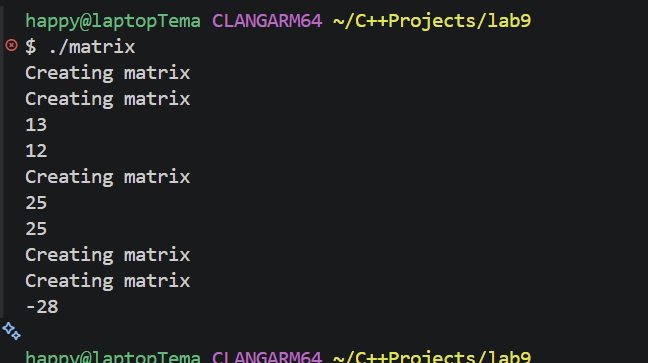
\includegraphics[width=0.85\textwidth]{lab9_1}
    \captionsetup{justification=centering}
    \captionof{figure}{Результат работы программы}
\end{center}

\section{Вывод}
В данной лабораторной работе был получен навык перегрузки операций
\end{document}